\documentclass[12pt, titlepage, letterpaper]{article}
%\documentclass[12pt, letterpaper, titlepage]{article}

\usepackage{amsmath}
\usepackage{booktabs}
\usepackage{amsthm}
\usepackage{graphicx}
\usepackage[margin=1in]{geometry}
\usepackage{hyperref}
\hypersetup{colorlinks = true, linkcolor = blue, citecolor=blue, urlcolor = blue}
\usepackage{natbib}
\usepackage{enumitem}
\usepackage{setspace}


\usepackage[]{lineno}
\linenumbers*[1]
% %% patches to make lineno work better with amsmath
\newcommand*\patchAmsMathEnvironmentForLineno[1]{%
 \expandafter\let\csname old#1\expandafter\endcsname\csname #1\endcsname
 \expandafter\let\csname oldend#1\expandafter\endcsname\csname end#1\endcsname
 \renewenvironment{#1}%
 {\linenomath\csname old#1\endcsname}%
 {\csname oldend#1\endcsname\endlinenomath}}%
\newcommand*\patchBothAmsMathEnvironmentsForLineno[1]{%
 \patchAmsMathEnvironmentForLineno{#1}%
 \patchAmsMathEnvironmentForLineno{#1*}}%

\AtBeginDocument{%
 \patchBothAmsMathEnvironmentsForLineno{equation}%
 \patchBothAmsMathEnvironmentsForLineno{align}%
 \patchBothAmsMathEnvironmentsForLineno{flalign}%
 \patchBothAmsMathEnvironmentsForLineno{alignat}%
 \patchBothAmsMathEnvironmentsForLineno{gather}%
 \patchBothAmsMathEnvironmentsForLineno{multline}%
}

% control floats
\renewcommand\floatpagefraction{.9}
\renewcommand\topfraction{.9}
\renewcommand\bottomfraction{.9}
\renewcommand\textfraction{.1}
\setcounter{totalnumber}{50}
\setcounter{topnumber}{50}
\setcounter{bottomnumber}{50}

\newcommand{\jy}[1]{\textcolor{blue}{JY: (#1)}}
\newcommand{\eds}[1]{\textcolor{red}{EDS: (#1)}}
\newcommand{\mc}[1]{\textcolor{green}{MC: (#1)}}

% NOTE: To produce blinded version, replace "0" with "1" below.
\newcommand{\blind}{1]}

\begin{document}
%\maketitle

\title{Nonparametric Block Bootstrap Kolmogorov-Smirnov Goodness-of-Fit Test}
  \author{Mathew Chandy %\\
%   \href{mailto:mathew.chandy@uconn.edu}
%   {\nolinkurl{mathew.chandy@uconn.edu}}\\
%  Elizabeth Schifano\\
%  Jun Yan\\
%  Xianyang Zhang\\
} 


\maketitle


\begin{abstract}

The Kolmogorov-Smirnov (KS) test is a widely used statistical test that
assesses the conformity of a sample to a specified distribution. Its efficacy,
however, diminishes with serially dependent data and when parameters
within the hypothesized distribution are unknown. For independent data,
parametric and nonparametric bootstrap procedure are available to adjust for
estimated parameters. For serially dependent stationary data, parametric
bootstrap has been developed with a working serial dependence structure. A
counterpart for the nonparametric bootstrap approach, which needs a bias
correction, has not been studied. Addressing this gap, our study introduces a
bias correction method employing a nonparametric block bootstrap, which
approximates the distribution of the KS statistic accounting for unspecified
serial dependence and unspecified parameters. We assess its effectiveness
through simulations, scrutinizing both its size and power. The practicality of
our method is further illustrated with an examination of stock returns from the 
S\&P 500 index, showcasing its utility in real-world
applications.

\bigskip
\noindent{\sc Keywords}:
bias-correction; 
serial dependence;
time series. 
\end{abstract}

\doublespace 


\section{Introduction}
\label{sec:intro}

The standard one-sample Kolmogorov-Smirnov (KS) test is widely
recognized as an effective good-of-fit test for continuous distributions.
Consider $X_1, ..., X_n$, a random sample of size~$n$ from some continuous
distribution and the null hypothesis $H_0$ that $X_i$'s follow a specific
hypothesized distribution~$F(x; \theta_0)$, where $\theta_0$ are the 
specified parameters
of the hypothesized distribution family.
If we let $F_n(t) = \sum_{i=1}^n I(X_i \le t) / n$ be the empirical cumulative
distribution function of the sample, where $I(\cdot)$ is the indicator
function, the KS test statistic takes the form
\begin{equation}
  \label{eq:ks_standard}
  T_n = \sqrt{n} \sup_x | F_{n}(x) - F(x; \theta_0)|.
\end{equation}
As sample size $n\to \infty$, the distribution of $T_n$ converges to that of the
absolute value of standard Brownian bridge, which is known as the Kolmogorov
distribution \citep{stephens1974edf}. This distribution function is
precisely computable using contemporary statistical software
\citep{marsaglia2003evaluating}. The versatility of the KS test allows its
application across various domains, such as analyzing cosmic microwave
background radiation \citep{naess2012application}, monitoring the count rate of
radioactive data \citep{aslam2020introducing}, gear condition monitoring
\citep{andrade2001gear}, studying images of breast cancer tumors
\citep{demidenko2004kolmogorov}, and examining financial markets
\citep{lux2001turbulence}.


Despite its widespread use, the KS test can be 
misapplied when its foundational assumptions are overlooked. The KS test 
assumes the data are independently and identically distributed and 
that the hypothesized distribution is continuous and fully specified without 
the need for parameter estimation. \citet{zeimbekakis2022misuses} examines
common misapplications of the one-sample KS test. One notable inappropriate
use is when the hypothesized distribution contains unspecified parameters.
In this case, the tests are generally constructed by substituting the unknown
parameters by their estimates, and the asymptotic null distribution of
the test statistic may depend in a complex way on the unknown parameters.
The problem of unspecified parameters can be handled by a parametric
bootstrap, where bootstrap samples of the test statistics are constructed from
samples generated from the fitted hypothesized distribution.
Alternatively, \citet{babu2004goodness} address this issue through a
nonparametric bootstrap method that corrects the bias in the asymptotic null
distribution.



Another prevalent misapplication of the KS test arises when data exhibit serial
dependence, which is often overlooked in analyses. For example, in an
investigation of performance variation in high-performance computing systems,
\citet{tuncer2019ieee} did not describe how or if they accounted for serial
dependence when applying the two-sample KS test.
The distribution of the test statistic under
the null hypothesis depends on the unknown parameters and unknown 
serial dependence. Therefore, the null distribution under dependence cannot be
used,
and the challenge is to approximate said distribution.
\citet{zeimbekakis2022misuses} proposed a semiparametric bootstrap
where the serial dependence structure is modeled via a working serial copula.


A particularly complex scenario arises when the distribution has unspecified
parameters, and the data are serially dependent. For this,
\citet{zeimbekakis2022misuses} also recommends a semiparametric bootstrap
approach, where the parameters of the hypothesized distribution and the serial
dependence both need to be estimated and their uncertainty accounted for,
but this could affect results if the estimated serial
dependence is too far from the truth. For this reason, a nonparametric method
is motivated.


Developing a fully nonparametric solution for the KS 
tests in the presence of serially dependent data presents a significant 
challenge. The null distribution's characteristics are intricately linked to 
the structure of the serial dependence, which can vary widely in practical 
situations. Employing a nonparametric bootstrap would necessitate defining a 
specific model for this dependence, despite the primary focus being on 
evaluating the marginal distribution of a stationary series. To date, a bias 
correction method for block bootstrap, akin to the nonparametric bootstrap
approach of \citet{babu2004goodness} for independent data,
has not been established. This study seeks 
to bridge this gap by introducing a bias correction technique for the 
nonparametric block bootstrap, tailored for use in scenarios where the 
hypothesized distribution has unspecified parameters and the data 
exhibit serial dependence. Our approach reduces to that of
\citet{babu2004goodness} when the data are independent.


The remainder of this paper is structured as follows: 
Section~\ref{sec:methods} provides an overview of the block bootstrap 
procedure and introduces the bias correction methodology for the 
nonparametric block bootstrap KS test. Section~\ref{sec:simu} is divided 
into two parts; initially, we evaluate the KS test's ability to maintain 
its size, i.e., its consistency in not rejecting the null hypothesis when 
it is indeed true. Subsequently, we examine the test's power, assessing 
whether it can reject the null hypothesis when it is false. Practical 
applications of our method are presented in Section~\ref{sec:real}, where 
we apply the approach to analyze if S\&P 500 index stock return
data adheres to either the Normal or the Student's $t$ distribution. The 
paper concludes with Section~\ref{sec:conclusion}, offering final thoughts 
and remarks.


\section{Methods}
\label{sec:methods}

Consider a stationary time series $\{X_t: t = 1, \ldots, n\}$ with length~$n$.
We are interested in testing whether or not $X_t$ follows a distribution in a
parametric family of distribution~$F$ indexed by a parameter
vector~$\theta$. That is, the null hypothesis is
\[
  H_0: X_t \sim F(\cdot \mid \theta), \quad t = 1, \ldots, n,
\]
for some unspecified parameter $\theta$.
The alternative hypothesis $H_A$ is that the marginal distribution of $X_t$ does
not follow~$F$ for any parameter value~$\theta$. This is a challenging situation
because both the parameters and the serial dependence structure are unknown.

\subsection{Kolmogorov--Smirnov Test}

First, let us review how the KS statistic is computed for an independent
sample with fitted parameters. Let $\hat\theta_n$ denote the parametrically
fitted parameters, which can be obtained from any consistent estimator with
asymptotic normality properties,  Let $F_n$ be the empirical distribution
function based on $X_1,...,X_n$.
Define 
\begin{equation*}
Y_n(x; \hat\theta) = \sqrt{n}(F_n(x) - F(x; \hat\theta_n)).
\end{equation*}
Then, the one-sample KS goodness of fit statistic is 
\begin{equation*}
T_n := \sup_x|Y_n(x; \hat\theta)|.
\end{equation*}


Because of the estimation uncertainty in $\hat\theta_n$, the asymptotic
distribution of $Y_n$ is no longer distribution-free. This is in contrast to the
case where $\theta$ is known.  Note that
\begin{equation*}
Y_n(x; \hat\theta) = \sqrt{n}(F_n(x) - F(x)) - 
\sqrt{n}(F(x; \hat\theta_n) - F(x)).
\end{equation*}
When $\hat\theta_n$ is replaced with $\theta$, as in the standard KS testing
situation, the second term vanishes, and $T_n$ converges in distribution to that
of $\sup_t | B(F(t)) |$, where $B(\cdot)$ is the standard Brownian bridge
\citep{kolmogorov1933sulla}. With $\hat\theta_n$ in place of $\theta$, the
second term leads to a bias in the Brownian bridge, which was addressed by
\citet{babu2004goodness}.


When $\{X_t: t = 1, \ldots, n\}$ are further serially dependent, the statistics
$T_n$ still provides a reasonable metric for deviation from the null
hypothesis. Nonetheless, the asymptotic distribution of $T_n$ cannot be fixed
even with the bias correction of \citet{babu2004goodness}, because the
correction requires independent sample.

\subsection{Nonparametric Bootstrap for Independent Data}

Continue with the case where $X_i$'s are independent but the parameters
are unspecified. Denote by
$F^{(b)}_n$ the empirical distribution of the $b$th bootstrap sample and let
$\hat\theta^{(b)}_n$ be the parameter estimate based on the $b$th bootstrap 
sample. 
Using the bootstrap (asymptotic) theory, we can approximate the distribution of
$\sqrt{n}(F_n(x) - F(x))$ and $\sqrt{n}(F(x; \hat\theta_n) - F(x))$
by that of $\sqrt{n}(F^{(b)}_n(x) - F_n(x))$ and
$\sqrt{n}(F(x; \hat\theta^{(b)}_n) - F(x; \hat\theta_n))$, respectively.
Therefore, if we define
\begin{align*}
Y^{(b)}_n(x) &= \sqrt{n}(F^{(b)}_n(x) - F_n(x)) - 
               \sqrt{n}(F(x; \hat\theta^{(b)}_n) - F(x; \hat\theta_n)) \\
             &= \sqrt{n}(F^{(b)}_n(x) - F(x; \hat\theta^{(b)}_n)) - 
               \sqrt{n}(F_n(x) - F(x; \hat\theta_n)),
\end{align*}
then $T^{(b)}_n := \sup_x|Y^{(b)}_n(x)|$ is the bootstrap statistic that is 
expected to approximate the distribution of $T_n$. We note that the term
$\sqrt{n}(F_n(x) - F(x; \hat\theta_n))$ is exactly the bias term considered in 
\citet{babu2004goodness}.


In summary, the procedure of the nonparametric bootstrap KS test for independent
sample is 
summarized as follows. Repeat the following steps for $b \in \{1, ..., B\}$.
\begin{enumerate}
\item
  Generate $X^{(b)}_1,...,X^{(b)}_n$ by applying basic bootstrap 
  on the original sample as
  defined previously.
\item
  Fit $F_\theta$ to $X^{(b)}_1,...,X^{(b)}_n$ and obtain estimate 
	$\hat\theta^{(b)}_n$ of $\theta$.
\item
  Obtain the empirical distribution function $F^{(b)}_n$ of
  $X^{(b)}_1,...,X^{(b)}_n$. 
\item
  Calculate bootstrap KS statistic
  \[
    T^{(b)}_n = \sup_x | \sqrt{n}\left(F^{(b)}_n(x) 
    - F(x; \hat\theta^{(b)}_n)\right) - B_n(x) |.
  \]
  where 
  $B_{n}(x) = \sqrt{n}(F_n(x) - F(x; \hat\theta_n))$ is the known
  bias term.
\end{enumerate}


The p-value of the basic bootstrap KS test can be approximated
as $p = \sum_{b=1}^B I\{T^{(b)}_n > T_n\} / B$.


\subsection{Nonparametric Block Bootstrap for Stationary Series}

We now consider the case where $X_i$'s are realizations from a time series and
$X^{(b)}_1,...,X^{(b)}_n$ are generated by block bootstrap for 
$b \in \{1, \ldots, B\}$.  
Block-bootstrap can be done with overlapping or moving blocks.
Define moving blocks (assuming $l > 1$) as:
\begin{equation*}
Z_j =
    \begin{cases}
        \{X_j, \ldots, X_{j + l - 1}\}, & j = 1, \dots, n - l + 1,\\
        \{X_j, \ldots, X_n, X_1, \ldots, X_{j-n+l-1}\}, & j = n - l
        + 2 ,\dots, n.
    \end{cases}
\end{equation*}
A common 
function for block size that is considered optimal is 
$l = \lceil n^{1/3} \rceil$ \citep{buhlmann1999block},  
which was adopted in this study.
Now we draw $k$ blocks from the $(n - l + 1)$ blocks 
of $Z_j$'s with replacement and then align them in the order they were picked to
form a block bootstrap sample. If $n$ is not a multiple of~$l$, the last block 
selected will be reduced in size so that the final size of the block bootstrap 
sample is $n$.


Continuing using the notation in the independent case,
we use $F^{(b)}_n$ and $\hat\theta^{(b)}_n$ for the empirical distribution and
the estimated parameters based on the $b$th bootstrap sample,
$b = 1, \ldots, B$.
We then use block bootstrap to approximate the asymptotic distribution of
the KS statistic under $H_0$. In particular, we
use the distribution of $\sqrt{n}(F^{(b)}_n(x) - E[F^{(b)}_n(x)])$
as an approximation of the distribution of
$\sqrt{n}(F_n(x) - F(x))$, and the distribution of 
$\sqrt{n}(F(x; \hat\theta^{(b)}_n) - F(x; E[\hat\theta^{(b)}_n]))$ as
an approximation of the distribution of $\sqrt{n}(F(x; \theta_n) - F(x))$.
The expected values $E[F^{(b)}_n(x)]$ and
$E[\hat\theta^{(b)}_n]$ can be approximated by, respectively,
$E_n[F^{(b)}_n(x)] = \frac{1}{B}\sum_{b = 1}^BF^{(b)}_n(x)$ and
$E_n[\hat\theta^{(b)}_n]  =  \frac{1}{B}\sum_{b = 1}^B\hat\theta^{(b)}_n$.


Then, we can define
\begin{align*}
  Y^{(b)}_n(x) &= \sqrt{n}(F^{(b)}_n(x) - E[F^{(b)}_n(x)]) - 
             \sqrt{n}(F(x; \hat\theta^{(b)}_n) - F(x; E[\hat\theta^{(b)}_n)]) \\
           &= \sqrt{n}(F^{(b)}_n(x) - F(x; \hat\theta^{(b)}_n)) -
             \sqrt{n}(E[F^{(b)}_n(x)] - F(x; E[\hat\theta^{(b)}_n])),
\end{align*}
and $T^{(b)}_n = \sup_x|Y^{(b)}_n(x)|$. Each $T_n^{(b)}$,
$b =1, \ldots, B$, is considered a draw from a distribution that approximates
the distribution of $T_n$. Therefore, the p-value of the observed statistic
$T_n$ can be assessed by positioning it agains the empirical distribution of
$T_n^{(b)}$, $b = 1, \ldots, B$.


In summary, the procedure of the nonparametric block bootstrap test is 
summarized as follows. Repeat the following steps for $b \in \{1, ..., B\}$.
\begin{enumerate}
\item
  Generate $X^{(b)}_1,...,X^{(b)}_n$ by applying moving block bootstrap 
  on the original sample as
  defined previously.
\item
  Fit $F_\theta$ to $X^{(b)}_1,...,X^{(b)}_n$ and obtain estimate 
	$\hat\theta^{(b)}_n$ of $\theta$.
\item
  Obtain the empirical distribution function $F^{(b)}_n$ of
  $X^{(b)}_1,...,X^{(b)}_n$. 
\item
  Calculate bootstrap KS statistic
  \[
    T^{(b)}_n = \sup_x | \sqrt{n}\left(F^{(b)}_n(x) 
    - F(x; \hat\theta^{(b)}_n)\right) - B_n(x) |.
  \]
  where 
  $B_{n}(x) = \sqrt{n}(E[F^{(b)}_n(x)] - 
  F(x; E[\hat\theta^{(b)}_n]))$ is the known
  bias term.
\end{enumerate}


The p-value of the block bootstrap KS test can be approximated
as $p = \sum_{b=1}^N I\{T^{(b)}_n > T_n\} / B$.


\section{Simulation Studies}
\label{sec:simu}

In this simulation study, our objective is twofold: firstly, to demonstrate that
under the null distribution, our test rejects the null hypothesis ($H_0$) 
approximately at the specified significance level. Secondly, we aim to
illustrate that under the alternate distribution, our test reliably rejects
$H_0$ at a high frequency. The fulfillment of both these criteria would indicate
the method's efficacy.


\subsection{Size}
We first must evaluate whether this method works when $H_0$ is true. To
test this, we can
generate a simulated sample $X_t$ with a certain marginal distribution 
$F_\theta$,
and use our method to test if $X_t$ indeed has the marginal distribution $F$ 
with some unknown $\theta$. If the test holds its size, the 
p-value
of the test should be uniformly distributed between 0 and 1. We must try the
method with different marginal distributions to ensure that it is robust.
In order for the method to work, a large sample size may be necessary. 


We generated time series with marginal distributions $N(8, 8)$ and
$\Gamma(8, 1)$ with Kendall's
$\tau \in \{-.75, -.5, -.25, 0, .25, .5, 75\}$, and
sample size $n \in \{100, 200, 400, 800\}$. Kendall's $\tau$ was chosen as a
measure of serial dependence as it does not vary between two different 
marginal distributions.
To generate the samples to which our
method would be applied, we simulated a time series $W_t$ from a 1st 
order autoregressive (AR(1)) process:
\begin{equation*}
W_t = \phi X_{t-1} + \epsilon_t,
\end{equation*}
where $\phi$ is an autoregressive coefficient, and $\epsilon_t$ is a series of
independent errors from a normal distribution with mean zero and variance
$\sigma_{\epsilon}^2$. The strength of the serial dependence is controlled by
$\phi$, which was set to five levels: 
$\{-0.924, -0.707, -0.383, 0, 0.383, 0.707, 0.924\}$, as these
correspond to the desired values for $\tau$. First, we generated a
marginal $N(8, 8)$ by marginally transforming $W_t$ by
\begin{equation*}
X_t = F^{-1}[\Phi(W_t)],
\end{equation*}
\jy{The language issues are more than I expected. Please do a careful proofread,
  now that you are more experienced.}
where $F^{-1}(p)$ is the quantile function for the $N(8, 8)$ 
distribution and $\Phi$ is the distribution function of the standard normal
distribution.
Then we generated a marginal gamma series by the same procedure, but
replacing $F^{-1}(p)$ with the quantile function for the $\Gamma(8, 1)$
distribution.
After the transformation
to the marginal gamma distribution, the autocorrelations are
\[
  \{-0.884, -0.686, -0.389, -0.033, 0.327, 0.639, 0.861\}.
\]


These distributions
were chosen to compare results on normal and non-normal
error structures. The specific parameters were chosen because the distributions 
are very similar and their
first two moments are the same. 
For the purposes of 
evaluating if the test holds it size, when $X_t \sim N(8, 8)$, we tested that the 
marginal distribution is from the
Normal family, or 
$X_t \sim N(\cdot \mid \mu, \sigma^2), \quad t = 1, \ldots, n$
for some unspecified $\mu$ and $\sigma$. When $X_t \sim \Gamma(8, 1)$, we tested
that the marginal distribution family is from the Gamma family,
or
$X_t \sim \Gamma(\cdot \mid \alpha, \beta), \quad t = 1, \ldots, n$.
for some unspecified $\alpha$ and $\beta$.
For the block
bootstrap step,
we used $B = 1000$ and $l = \lceil n^{1/3} \rceil$.
For each setting for $F$, $\tau$, and $n$, we replicate the method 1000 times 
to get the distribution of the p-values $p_r$
for the test when applied to samples from the same data generating process.


Using R packages \textsl{qqplotr} and \textsl{ggplot2} \citep{qqplotr, ggplot2},
we constructed Q-Q plots of the distribution of the p-values to see if they are
uniformly distributed. If the distribution of the p-values is uniform, the
points will be aligned with the diagonal line. This 
indicates that under the null hypothesis, our method will only reject the $H_0$
at the rate of the significance level.
\jy{Describe the table not zoomed-in figure.}\mc{addressed}
A table of the rejection rates for each scheme
also provided.

\begin{figure}[tbp]
  \centering
  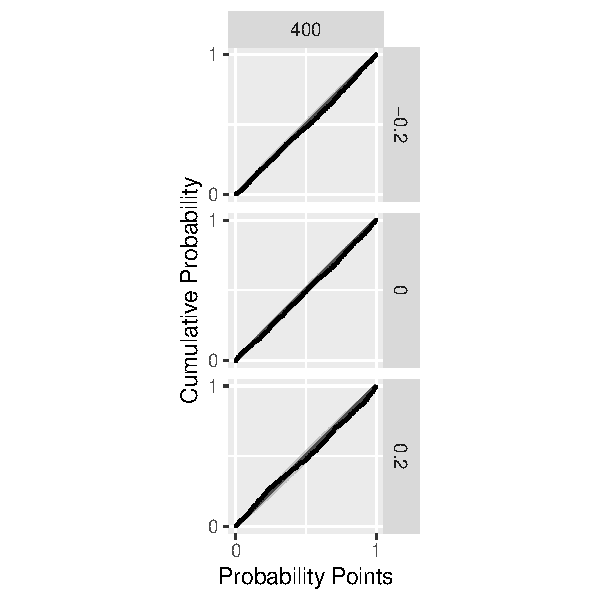
\includegraphics[width = \textwidth]{figures/normal}
  \caption{A Q-Q plot of the p-values testing that a distribution
  generated from a $N(8,8)$ data generating process is normal.}
  \label{fig:normal}
\end{figure}


\begin{figure}[tbp]
  \centering
  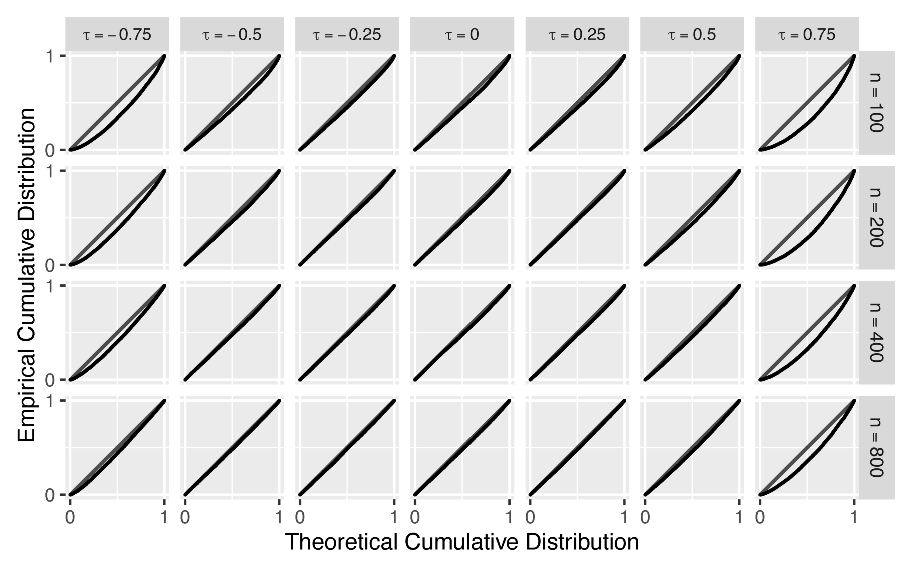
\includegraphics[scale=1]{figures/gamma}
  \caption{A Q-Q plot of the p-values testing that a distribution
  generated from a $\gamma(8,1)$ data generating process is gamma distributed.}
  \label{fig:gamma}
\end{figure}

% latex table generated in R 4.3.0 by xtable 1.8-4 package
% Mon May  6 14:42:26 2024
\begin{table}[ht]
\centering
\caption{Rejection rates for test that $N(8, 8)$ is indeed
                   normally distributed for
                   different values of AR(1) coefficient and for different 
                   significance levels.} 
\label{table:rr_norm}
\begin{tabular}{rllrrrrrrr}
  \hline
 & $n$ & $\alpha$ & $\tau = -0.75$ & $\tau = -0.5$ & $\tau = -0.25$ & $\tau = 0$ & $\tau = 0.25$ & $\tau = 0.5$ & $\tau = 0.75$ \\ 
  \hline
1 & 100 & 0.01 & 0.052 & 0.013 & 0.007 & 0.011 & 0.009 & 0.013 & 0.058 \\ 
  2 & 100 & 0.05 & 0.138 & 0.061 & 0.038 & 0.059 & 0.054 & 0.083 & 0.178 \\ 
  3 & 100 & 0.1 & 0.238 & 0.125 & 0.089 & 0.124 & 0.102 & 0.152 & 0.272 \\ 
  4 & 200 & 0.01 & 0.043 & 0.009 & 0.006 & 0.017 & 0.011 & 0.018 & 0.062 \\ 
  5 & 200 & 0.05 & 0.130 & 0.058 & 0.041 & 0.051 & 0.053 & 0.061 & 0.175 \\ 
  6 & 200 & 0.1 & 0.202 & 0.120 & 0.101 & 0.107 & 0.110 & 0.125 & 0.266 \\ 
  7 & 400 & 0.01 & 0.037 & 0.011 & 0.009 & 0.014 & 0.013 & 0.009 & 0.043 \\ 
  8 & 400 & 0.05 & 0.109 & 0.047 & 0.052 & 0.061 & 0.044 & 0.064 & 0.133 \\ 
  9 & 400 & 0.1 & 0.174 & 0.099 & 0.098 & 0.108 & 0.099 & 0.123 & 0.212 \\ 
  10 & 800 & 0.01 & 0.023 & 0.011 & 0.008 & 0.011 & 0.011 & 0.011 & 0.038 \\ 
  11 & 800 & 0.05 & 0.088 & 0.043 & 0.040 & 0.055 & 0.042 & 0.053 & 0.125 \\ 
  12 & 800 & 0.1 & 0.166 & 0.097 & 0.095 & 0.102 & 0.107 & 0.109 & 0.196 \\ 
   \hline
\end{tabular}
\end{table}



% latex table generated in R 4.3.0 by xtable 1.8-4 package
% Sat May 18 07:28:05 2024
\begin{table}[ht]
\centering
\caption{Empirical sizes for the test that sample follows its true
                    distribution family for
                   different values of AR(1) coefficient and for different 
                   significance levels.} 
\label{table:rr_gamma}
\begin{tabular}{llrrrrrrr}
  \hline
$n$ & $\alpha$ & $\tau = -0.75$ & $\tau = -0.5$ & $\tau = -0.25$ & $\tau = 0$ & $\tau = 0.25$ & $\tau = 0.5$ & $\tau = 0.75$ \\ 
  \hline
100 & 0.01 & 4.8800 & 1.4200 & 1.1700 & 1.2400 & 1.1100 & 1.6100 & 5.7600 \\ 
  100 & 0.05 & 2.8500 & 1.2820 & 1.2220 & 1.1700 & 1.1780 & 1.4640 & 3.3740 \\ 
  100 & 0.10 & 2.2410 & 1.2240 & 1.1470 & 1.1750 & 1.1500 & 1.3750 & 2.6790 \\ 
  200 & 0.01 & 4.0800 & 1.0000 & 0.8900 & 1.2200 & 1.1600 & 1.4300 & 6.0800 \\ 
  200 & 0.05 & 2.5100 & 1.1180 & 1.0140 & 1.0680 & 1.1160 & 1.2900 & 3.3800 \\ 
  200 & 0.10 & 1.9910 & 1.1050 & 1.0220 & 1.0480 & 1.0720 & 1.2330 & 2.6640 \\ 
  400 & 0.01 & 3.1400 & 0.9700 & 1.1400 & 0.9400 & 1.0300 & 1.3100 & 4.3000 \\ 
  400 & 0.05 & 2.0040 & 0.9640 & 1.0420 & 1.0620 & 1.1220 & 1.2360 & 2.8080 \\ 
  400 & 0.10 & 1.6970 & 1.0250 & 1.0660 & 1.0180 & 1.1000 & 1.1770 & 2.2320 \\ 
  800 & 0.01 & 2.4900 & 0.9200 & 1.1300 & 1.1200 & 1.0000 & 1.1300 & 3.8100 \\ 
  800 & 0.05 & 1.8040 & 0.9760 & 1.0640 & 1.0220 & 1.0860 & 1.1960 & 2.4740 \\ 
  800 & 0.10 & 1.5610 & 1.0240 & 1.0720 & 1.0340 & 1.0670 & 1.1770 & 1.9970 \\ 
   \hline
\end{tabular}
\end{table}



From Figures~\ref{fig:normal} and \ref{fig:gamma}, we can observe that 
the extent to which the p-values are uniformly distributed
is dependent on the sample size and the level of serial 
dependence.
A small sample size like $n = 100$ or $200$ seems adequate when Kendall's
$\tau$ is lower than 0.25. For Kendall's $\tau \geq 0.5$, a sample larger than
$n = 200$ seems necessary for the p-values to be normally distributed. For
Kendall's $\tau \geq 0.75$, a sample larger than $n = 800$ appears to be 
necessary, as the p-values are not aligned with the line in any of the Q-Q 
plots. This
is not necessarily a cause for concern, as (for normal margins)
a Kendall's $\tau$ corresponds to
a $\phi$ of 0.924, which is very high.
Additionally, positive serial dependence appears to misalign the distribution
of the p-values more so than negative serial dependences of the same strength.
Results are very similar for normal and gamma margins.
\jy{Summarize findings in bullet points before forming text.}


From Tables~\ref{table:rr_norm} and \ref{table:rr_gamma}, we can observe 
that the agreement between empirical size (rejection rate)
and nominal size (the
significance level) improves as sample size increases, but for $\tau = -0.75$
and $\tau = 0.75$, a sample size larger than 800 seems to be necessary for that 
agreemet to be reached. Using the criteria of approximate agreement between 
empirical size and nominal size, we can say that our approach is working 
for $-0.25 < \tau < 0.25$ for $n > 100$. However a larger sample size seems 
necessary, greater than 400 perhaps, for $\tau$ as strong as $0.5$. To 
summarize, for weaker dependence, our method works without need for a 
particularly
large sample size, whereas for moderate dependence, a larger sample size may 
be required. Because $\tau$ is typically less than 0.5, it is still reasonable
to
recommend our method with a smaller sample size.





\subsection{Power}
The power of the proposed test is investigated with data generated from
distributions that are not in the hypothesized distribution family. If the test
is indeed powerful, we would ideally want the probability of
rejecting $H_0$ when $H_0$ is false\jy{beta has been
  used. Discuss in terms of power: the probability of rejecting $H_0$ when $H_0$
  is false.}\mc{addressed}
to be 1, but we
expect it to be generally high. Again, we must try the method with different
marginal distributions to ensure that it is robust.



\jy{Description too wordy, Be concise. Basically generate data from one
  distribution but test for the other distribution.}\mc{addressed}
We generated the same scheme of time series as we did when testing size, but
tested that the time series was from the other distribution.
Because the support of $N(8, 8)$ is
$(-\infty, \infty)$, but the support of $\Gamma(8, 1)$ is $(0, \infty)$, we used
the \textsl{truncdist} package \citep{truncdist} to truncate the series at 
values less than or equal to 0 when testing that $N(8, 8)$ sample was
from $\Gamma(8, 1)$. For each setting for $F$, $\tau$, and $n$, we replicate the 
method $1000$ times 
to obtain a p-value $p_r$ for each $r \in \{1, \ldots, 1000\}$.


\jy{alpha has been used as gamma parameters. This is not necessary, Just say we
  checked the power when the significance level is .05.}\mc{addressed}
We can compute a rejection rate 
at a nominal significance level of 0.05.
Additionally, we can construct a 95\% confidence interval for 
this rate. Below are tables containing rejection rates showcasing the 
differences when simulation settings are changed.


\begin{figure}[tbp]
  \centering
  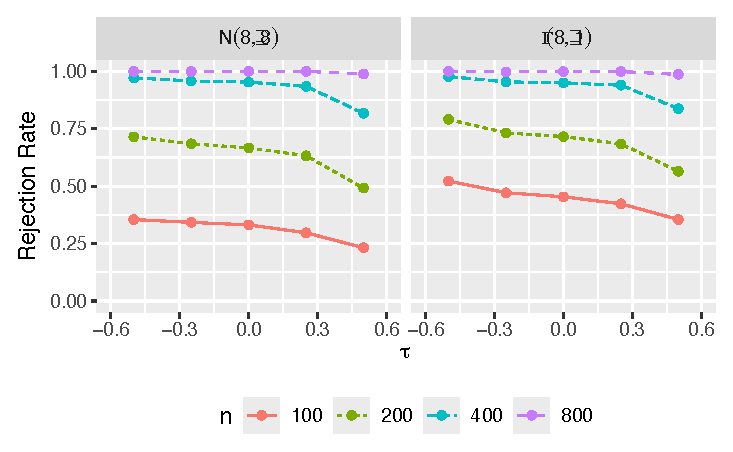
\includegraphics[scale=1]{figures/rr}
  \caption{A plot of the rejection rates as a function of $\tau$ for
 $n \in \{100, 200, 400, 800\}$ and marginal distribution 
 $\in \{N(8,8), \Gamma(8,1)\}$.}
  \label{fig:rr}
\end{figure}


Figure~\ref{fig:rr} displays the empirical power curve of the test at
significance level 0.05 as the lag-1 Kendall's~$\tau$ increases from
$-0.5$ to $0.5$. We omitted -0.75 and 0.75 from this study because we already 
found that our method doesn't work under the null hypothesis for such high
dependence levels. It appears that rejection rate seems to decline as $\tau$ 
increases. Using $n \geq 400$ seems to be good enough
if $\tau < 0.5$, but using a $n \geq 800$ will result in 
rejection rates close to 1 for $0.5 < \tau < 0.5$.
Results for $n \geq 400$
do not appear to be to different when comparing gamma and normal 
margins, indicating that the method is robust to the marginal distribution.
The rejection rates for $n = 800$ are very 
high (almost 1), indicating that under $H_A$, the test is very powerful 
(low probability of failed rejection $\beta$) when a large enough
sample size is used.


\section{Real Data Examples}
\label{sec:real}

Using the \textsl{tseries} package  \citep{tseries}, 
we gathered daily closing prices for the S\&P 500 index from January 1st, 2020
to December 31st, 2023. Daily returns were obtained by taking the difference in
the logarithm of the closing prices. The Kendall's $\tau$ for the series
was about -0.0298, indicating a very slight serial dependence.
Using our method, we tested that the daily returns are normally
distributed and Student's $t$ distributed 
with degrees of freedom $v \in \{30, 20, 10, 5, 4, 3, 2, 1\}$.
We tested the same hypotheses using 1) the
semiparametric bootstrap method shown by \citet{zeimbekakis2022misuses} which 
accounts for both serial dependence and unspecified parameters, 2)
nonparametric basic bootstrap bias correction developed by 
\citet{babu2004goodness}, and 3) the parametric bootstrap method shown
by \citet{zeimbekakis2022misuses}.
We used $B = 10,000$ bootstrap 
replicates in this analysis.
The p-values for these tests are highlighted in 
Table~\ref{table:SP5004}. 

\jy{Put them into one table; add results for paremetric bootstrap with
  Zeimbakakis' approach with serial dependence accounted for; label the methods
  as serial dependence accounted for and not accounted for, two methods
  (parametric and nonparametric) under each.}

\jy{Discuss the difference between the semiparametric bootstrap and the proposed
  nonparametric bootstrap. The semiparametric method depends on a working copula
  model for the serial dependence. If that is severely misspecified, I'd expect
  poor performance. The proposed method does not need to specify that dependence
  structure.}
\mc{addressed earlier}


% latex table generated in R 4.3.0 by xtable 1.8-4 package
% Fri Mar 15 20:41:15 2024
\begin{table}[ht]
\centering
\caption{P-values for 4 years of SP500 stock return 
                   data using different durations
  and different degrees of freedom for Student's t distribution.} 
\label{table:SP5004}
\begin{tabular}{rlllll}
  \hline
 & duration & df & block & basic & param \\ 
  \hline
1 & 4 & norm & 1e-04 & 0 & 0 \\ 
  2 & 4 & 30 & 0.0019 & 0 & 0 \\ 
  3 & 4 & 20 & 0.0027 & 0 & 0 \\ 
  4 & 4 & 10 & 0.0125 & 3e-04 & 3e-04 \\ 
  5 & 4 & 5 & 0.061 & 0.0222 & 0.0141 \\ 
  6 & 4 & 4 & 0.1037 & 0.0574 & 0.0499 \\ 
  7 & 4 & 3 & 0.3133 & 0.2759 & 0.2686 \\ 
  8 & 4 & 2 & 0.0418 & 0.0377 & 0.0443 \\ 
  9 & 4 & 1 & 0 & 0 & 0 \\ 
   \hline
\end{tabular}
\end{table}




\jy{Stock returns are known to be serially dependent and heavy-tailed. Search
  google scholar ``stylized facts of daily returns series'' and cite them.}
\mc{addressed}

While differences in p-values among different methods are expected, our analysis
reveals numerous instances where conclusions at the 0.05 significance level
using our method differ from those obtained using the methods proposed by
\citet{babu2004goodness} and \citet{zeimbekakis2022misuses}.
For example, when assessing the S\&P 500 series, our method fails to reject the
hypothesis that the series follows a Student's $t$ distribution with degrees of
freedom $v = 5$ with a p-value of 0.061. In contrast, 
the semiparametric method yields a p-value of 0.0192,
the basic nonparametric method
yields a p-value of 0.0222, and the parametric method yields a p-value of
0.0141. Although such differences are not guaranteed, this
instance highlights a disagreement in conclusions among methods for the S\&P 500
index.




\section{Concluding Remarks}
\label{sec:conclusion}

The Kolmogorov-Smirnov test stands as a crucial tool for researchers across
diverse fields, enabling comparisons of population distributions. This paper
introduces a variant of the test tailored for serially dependent data without
necessitating parameter specification.
Using simulation, we have shown that given a large enough sample of a time 
series and if the serial dependence is not too extreme, the block 
bootstrap KS test can appropriately fail to reject the null hypothesis when the
series follows the null distribution. In addition, when the marginal
distribution is not
the one hypothesized, the test is powerful. Notably, it demands a larger sample
size compared to basic bootstrap methods to avoid both type I and type II 
errors. Unsurprisingly,
the method performs better as the temporal dependence gets weaker. Through
simulation studies with Normal and Gamma-distributed data, we have shown that
that the method is robust. 


We have also 
demonstrated possible applications of this method to financial data.
Through comparison with the nonparametric
bootstrap bias correction developed by \citet{babu2004goodness}
and the parametric and semiparametric
bootstrap methods developed by \citet{zeimbekakis2022misuses}, we have 
underscored the importance of accounting for serial
dependence in choosing an appropriate methodology.
This method holds relevance for studies aiming to assess if a serially dependent
time series adheres to a hypothesized distribution in scenarios where parameters
are unknown or unspecified. Future studies could investigate
\jy{Too vague.}\mc{addressed}
the method's performance on different marginal distributions such
as the generalized extreme value distribution and
different dependence structures such as MA, ARMA, and ARIMA processes. Additionally, one could propose a 
similar method
for comparing two serially dependent methods. One could also apply the method
showcased
in this paper to fields like earthquake prediction and astronomy. 

\jy{summarize remarks in bullet points first. Let's talk on Tuesday.}

\bibliographystyle{asa}
\bibliography{citations}


\end{document}
%%% LocalWords: nonparametric semiparametric autocorrelation ARMA
%%% Local Variables:
%%% mode: latex
%%% TeX-master: t
%%% ispell-personal-dictionary: ".aspell.en.pws"
%%% fill-column: 80
%%% eval: (auto-fill-mode 1)
%%% End: